\section{Part 1}
\begin{enumerate}
    \item Based on the experimental observations where when the modulation index was increased the amplitude of the frequency components was increased, and the mathematical theory, it is observed that the amplitude of the relative frequency components grows in relation to the modulation index.

          Mathematically, it is known that the modulation index for an AM signal is given by:
          \begin{equation}
              m = kA_m
          \end{equation}

          Where $k$ is the transmitter sensitivity, and $A_m$ is the modulating signal amplitude, meaning that the modulation amplitude is proportional to the modulation index, while inversely proportional to the transmitter sensitivity.
    \item The modulation index can be computed from the equation found in the prelab, where the modulation index can be found using the maximum amplitude and the minimum amplitude.
          \begin{equation}
              m = \frac{A_{max} - A_{min}}{A_{max} + A_{min}}
          \end{equation}
          For 70\% modulation at the function generator:
          \begin{equation}
              m = \frac{4.32V - 0.8V}{4.32V + 0.8V} \simeq 0.68 \simeq 68\%
          \end{equation}
          For 50\% modulation:
          \begin{equation}
              m = \frac{3.76V - 1.28V}{3.76V + 1.28V} \eqsim 0.49 \eqsim 49\%
          \end{equation}
          For 120\% modulation:
          \begin{equation}
              m = \frac{5.52V + 0.48V}{5.52V - 0.48V} \eqsim 1.19 \eqsim 119\%
          \end{equation}
    \item The disadvantages of using a modulation index greater than 100\% lie in the distortion of the signal, as the carrier wave is not able to fully represent the modulating signal, therefore the envelope of the signal is distorted, making the signal unrecoverable.
\end{enumerate}

\section{Part 2}
\begin{enumerate}
    \item The spectrum in the oscilloscope for the 70\% modulation is shown to be 20KHz for the carrier wave, and 19.81KHz for the modulating wave. When plotting the FFT of the signal in theory using MATLAB, similar results are observed:
          \begin{figure}[H]
              \centering
              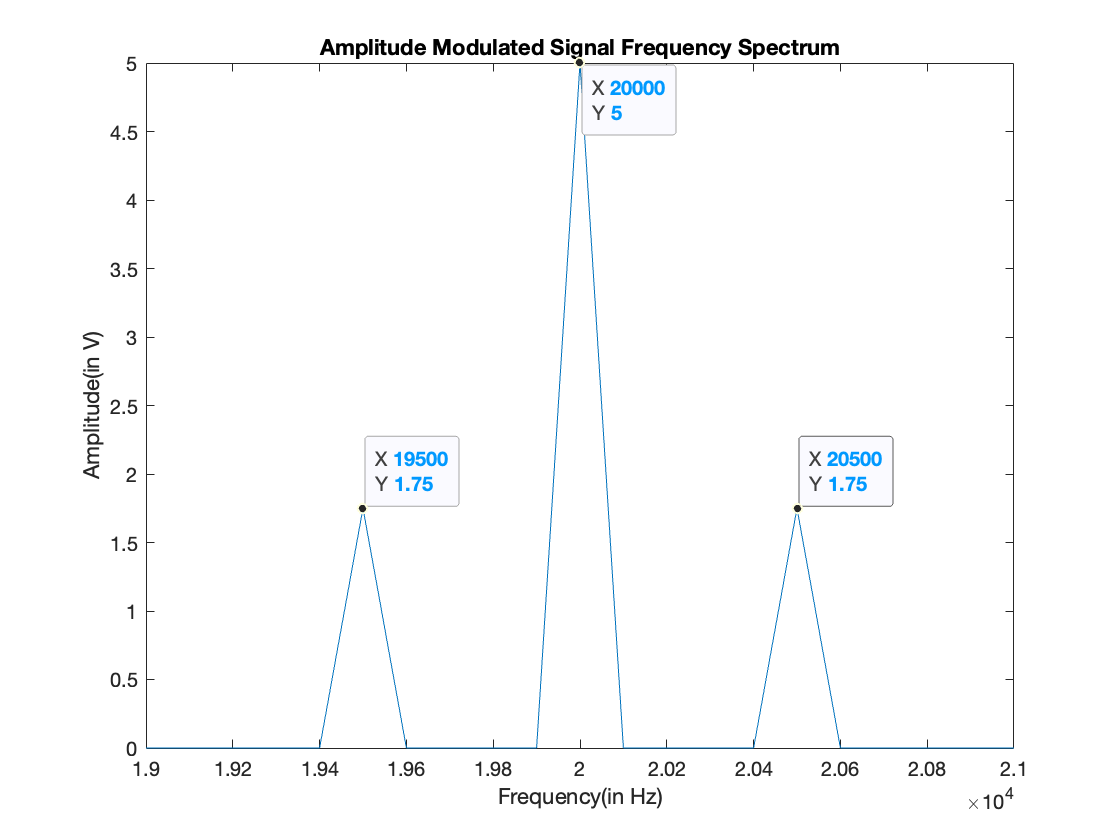
\includegraphics[width=0.5\textwidth]{images/evaluation_part2.png}
              \label{fig:evaluation_part2}
              \caption{Theoretical 70\% modulation index FFT, with the peaks at 19.5KHz, 20KHz, and 20.5KHz respectively}
          \end{figure}
    \item The function generator clearly generates a double-sideband signal, without suppressing the carrier as the carrier is observed in the fourier transform of the signal in the oscilloscope.
    \item When changing the carrier frequency of the signal, the spacing of the sidebands changes to move accordingly, as the modulating signal is convolved with the carrier signal.
    \item Changing the message frequency of the signal changes the width of the spectrum of the signal, as the modulating signal is convolved with the carrier signal and the width of the sidebands changes.
    \item The modulation index in the frequency spectrum can be found by taking the ratio between one of the sideband peaks amplitudes and the carrier peak amplitudes, so
          \begin{equation}
              m = \frac{4.15dB}{5.05dB} \simeq 0.82 \simeq 82\%
          \end{equation}
          This implies that the FFT of the signal as measured on the oscilloscope is not a perfect representation of the signal, as the modulation index is not 70\% as expected.
\end{enumerate}

\section{Part 3}
\begin{enumerate}
    \item The first order and the third order message signal as displayed in the oscilloscope show that the envelope of the signal is tracked better by the third order filter, with the first order filter not being able to track the amplitude peaks in order to track the envelope of the signal in the same manner.
    \item The first order filter is quite similar to what is observed in MATLAB, with the first order filter not being able to track the envelope of the signal with the same accuracy as the third order filter. The differences between the measurement and the simulation are due to the fact that the simulation is done using an ideal filter, while the measurement is done using a real filter, which has a non-ideal frequency response.
\end{enumerate}
